\documentclass[a4paper,12pt]{report}
\addtolength{\oddsidemargin}{-1.cm}
\addtolength{\textwidth}{2cm}
\addtolength{\topmargin}{-2cm}
\addtolength{\textheight}{3.5cm}
\newcommand{\HRule}{\rule{\linewidth}{0.5mm}}
\makeindex

\usepackage{longtable}
\usepackage[pdftex]{graphicx}
\usepackage{makeidx}
\usepackage{hyperref}
\hypersetup{
    colorlinks=true,
    linkcolor=blue,
    filecolor=magenta,      
    urlcolor=cyan,
}


% define the title
\author{Not-Like-This}
\title{ Nimbus Functional Requirements}
\begin{document}
\setlength{\parskip}{6pt}

% generates the title
\begin{titlepage}

\begin{center}
% Upper part of the page       

\includegraphics[width=1\textwidth]{./up-logo.jpg}\\[0.4cm]    
\textsc{\LARGE Department of Computer Science}\\[1.5cm]
\textsc{\Large COS 301 - Software Engineering}\\[0.5cm]
% Title
\HRule \\[0.4cm]

\includegraphics[width=0.05\textwidth]{./logo.png} 
{ \huge \bfseries Nimbus}

\includegraphics[width=0.05\textwidth]{./logo.png}\\[0.4cm] 
{ \huge \bfseries Functional Requirements}\\[0.4cm]
\HRule \\[0.4cm]
% Author and supervisor
\begin{minipage}{0.4\textwidth}
\begin{flushleft} \large
\emph{Authors:}
\end{flushleft}
\end{minipage}
\begin{minipage}{0.4\textwidth}
\begin{flushright} \large
\emph{Student number:}
\end{flushright}
\end{minipage}

\begin{minipage}{0.4\textwidth}
\begin{flushleft} \large
Jedd {Schneier}
\end{flushleft}
\end{minipage}
\begin{minipage}{0.4\textwidth}
\begin{flushright} \large
\emph{}
u13133064
\end{flushright}
\end{minipage}

\begin{minipage}{0.4\textwidth}
\begin{flushleft} \large
Daniel {King}
\end{flushleft}
\end{minipage}
\begin{minipage}{0.4\textwidth}
\begin{flushright} \large
\emph{}
u13307607
\end{flushright}
\end{minipage}

\begin{minipage}{0.4\textwidth}
\begin{flushleft} \large
Muller {Potgieter}
\end{flushleft}
\end{minipage}
\begin{minipage}{0.4\textwidth}
\begin{flushright} \large
\emph{}
u12003672
\end{flushright}
\end{minipage}

\vfill
% Bottom of the page
{\large \today}
\end{center}
\end{titlepage}
\footnotesize
%\input{declaration_of_originality.tex}
\normalsize

\renewcommand{\thesection}{\arabic{section}}
\newpage
\begin{center}
\textsc{\LARGE Software Requirements Specification and Technology Neutral Process Design}\\[1.5cm]
\textsc{\Large Nimbus AWS Network Visualiser/Main Project}\\[0.5cm]
Version: Version 1.0 Beta
For further references see \href{ https://github.com/u13133064/NotLikeThis}{gitHub}.
\today
\end{center}
\tableofcontents{}
\newpage
\section{Functional requirements}
\subsection{Introduction}
The Nimbus Amazon Web Services (AWS) network visualiser will be used to visualise a user's network within the AWS network, through their browser. The purpose of this document is to identify and explain all possible use cases associated with the visualiser and to show how the functional aspects of the visualiser interact with each other.
% \newpage
\subsection{Use case prioritiation}
\textbf{Critical} 
\begin{itemize}
  \item Log in/Log out
  \item Scan network
  \item Visualise network
  \item Get Node Connections
  \item Get Node information
\end{itemize}
\textbf{Important} 
\begin{itemize}
  \item Stop scan
  \item Resume scan
  \item Scan Up
  \item Scan Region
  \item Scan From
  \item Scan Instances
\end{itemize}
\textbf{Nice-To-Have} 
\begin{itemize}
  \item Load scan from local .json
  \item Save scan to local .json
\end{itemize}
\newpage
\subsection{Use case/Service contracts}
\begin{center}
  \begin{longtable}{| p{3cm} | p{4cm} | p{4cm} | p{4cm} |}
    \hline
    Use Case & Pre Condition & Post Condition & Description \\ 
    \hline \hline
    Log in/log out & The visualiser has to be connected to the internet in order to verify the information. Only a registered AWS user with a valid key and secret key may log into the system. Once the user is logged in he/she can then use the logout functionality to log out. & The user is logged in now and may begin making use of the visualisation server. & This use case provides a method for logging in to view a hierarchical representation of their network and log out once done.\\ 
    \hline
    Scan network & The visualiser must be connected to the internet in order to load the information from the server. The user must have instances in their network, that the server may scan. & The server continuously sends information of the instances to the browser, which are then stored by the browser. & This use case provides a method for loading the network representation from the AWS network and storing it on a browser. \\ 
    \hline
    Visualise Network &  The visualiser must be connected to the internet in order to load the information from the server. The user must have instances in their network, that the server may scan. The browser must have a feed from the server, that contain instance information. & As new node information is loaded into the browser, the browser will sequentially display them in a hierarchy.  &  This use case provides a method for reading information the browser has received and visualising it.\\ 
    \hline
    
    Get Node Connections &  aaa. & aaa.  &  aaa.\\ 
    \hline
     Get Node Infromation &  aaa. & aaa.  &  aaa.\\ 
    \hline
    
    Stop scan & The scan must be active. & The scan's execution is temporarily halted.  & This use case provides a method for temporarily halting an active scan.\\ \hline
    Resume scan & An active scan must have been stopped. & The scan resumes its execution. &  This use case provides a method for resuming a previously halted scan.\\ 
    \hline
	Scan Up & The scan must be active. & The direction of the scan is altered & This use case provides a way of changing the direction of the scan.\\ 
	\hline
    Scan Region & The scan must be active. & The scan refocuses and only scans instances that fall below a certain region. & This use case provides a way to only scan instances that belong to a specific AWS region.\\ \hline
    
    Scan From &  aaa. & aaa.  &  aaa.\\ 
    \hline
    Scan Instances &  aaa. & aaa.  &  aaa.\\ 
    \hline
    
    Load scan from local .json & A .json file with the correct formatting must be stored on the local device. & The browser processes the information on the .json and visualises it, as it would with a normal scan. & This case provides a way load network visualisations, without the need to scan it from the server.\\ \hline
    Save scan to local .json & The scan must be active/ finished. & A window appears that will save a .json file to the local device. The file is named with a time stamp, in order to avoid issues if multiple files are saved & This case provides a way to save a representation of the current scan, that can be loaded at a later date.\\ 
    \hline
  \end{longtable}
\end{center}
\newpage


\subsection{Required functionality}
\begin{itemize}
	% We need to add the correct pictures here. We must also give a description of the elements.
	\item \textbf{Log in/log out}
		\begin{flushleft}
		 Basically just say what this part does. 	
		\end{flushleft}
		\begin{center}
  	 	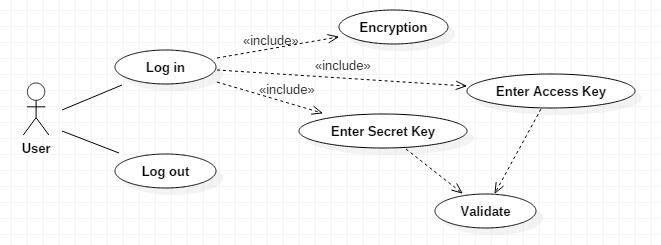
\includegraphics[width=1\textwidth] {./Diagrams/LoginUseCase.png}\\[0.4cm]    
		\end{center}

	\item \textbf{Scan network}
		\begin{flushleft}
			Basically just say what this part does.
		\end{flushleft}
		\begin{center}
  	 	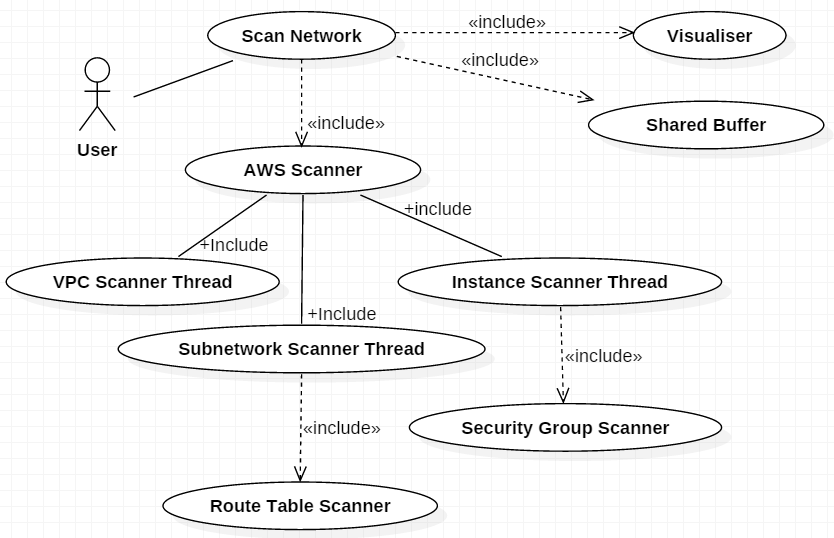
\includegraphics[width=1\textwidth] {./Diagrams/ScanNetworkUseCase.png}\\[0.4cm]    
		\end{center}

	\item \textbf{Get Node Information}
	\begin{flushleft}
		Basically just say what this part does.
	\end{flushleft}
	\begin{center}
		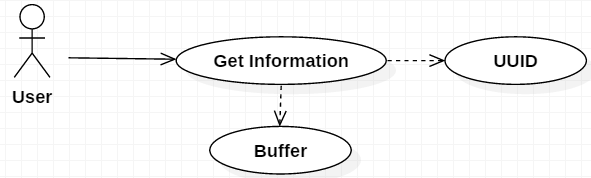
\includegraphics[width=1\textwidth] {./Diagrams/GetNodeInformationUseCase.png}\\[0.4cm]    
	\end{center}


	\item \textbf{Stop/Pause/Resume Scan}
	\begin{flushleft}
		Basically just say what this part does.
	\end{flushleft}
	\begin{center}
		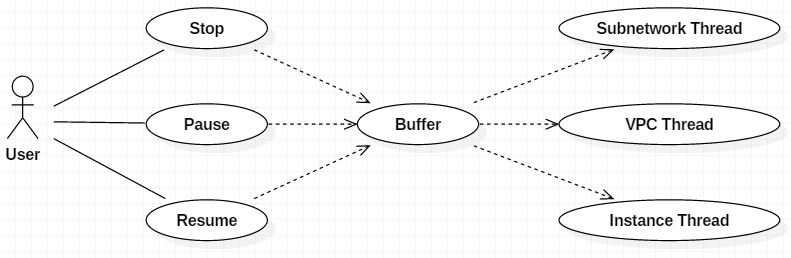
\includegraphics[width=1\textwidth] {./Diagrams/StopResumePauseUseCase.png}\\[0.4cm]    
	\end{center}

	\item \textbf{Scan From}
	\begin{flushleft}
		Basically just say what this part does.
	\end{flushleft}
	\begin{center}
		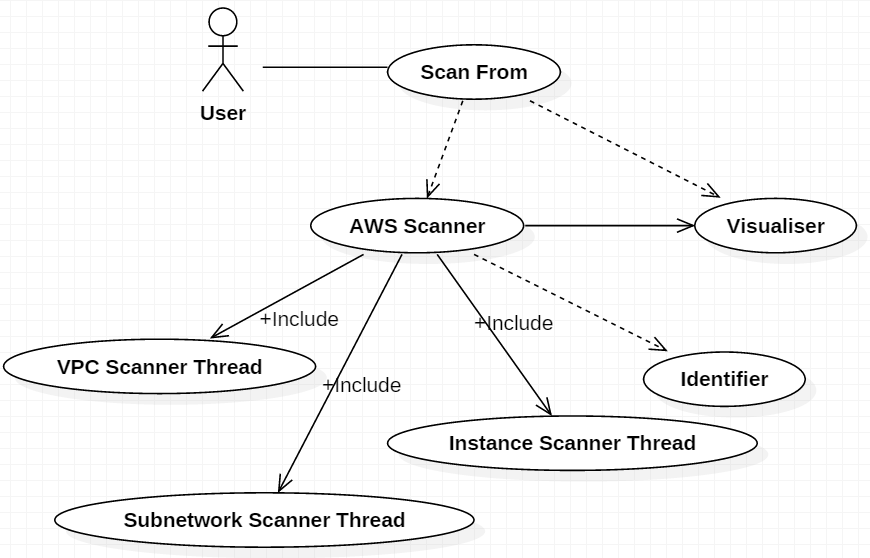
\includegraphics[width=1\textwidth] {./Diagrams/ScanFromUseCase.png}\\[0.4cm]    
	\end{center}

	\item \textbf{Scan Instances}
	\begin{flushleft}
		Basically just say what this part does.
	\end{flushleft}
	\begin{center}
		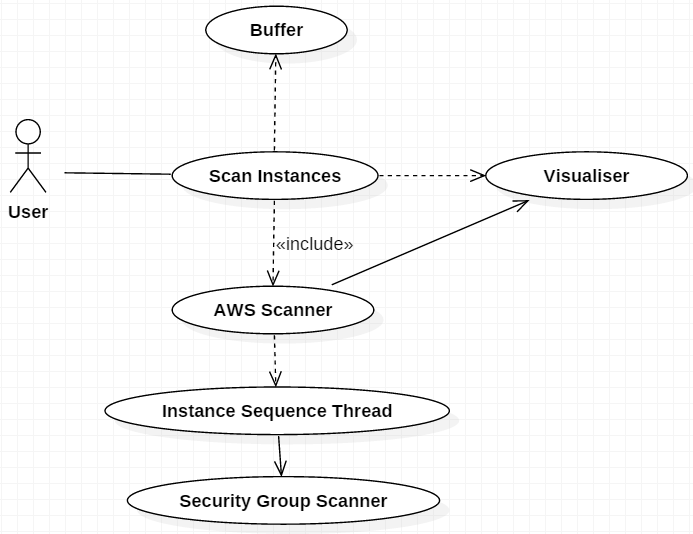
\includegraphics[width=1\textwidth] {./Diagrams/ScanInstancesUseCase.png}\\[0.4cm]    
	\end{center}

\end{itemize}
\newpage
\subsection{Process specification}
The processes followed when using some of the more important functions of the OnlyRugby app system are displayed below:
\begin{itemize}
	\item Log in/ log out
		\begin{center}
  	 	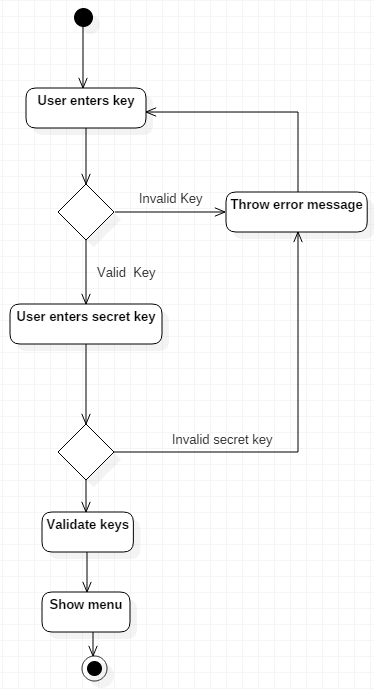
\includegraphics[width=0.6\textwidth] {./Diagrams/LoginSequence.png}\\[0.4cm]    
		\end{center}
	\item Scan network
		\begin{center}
  	  	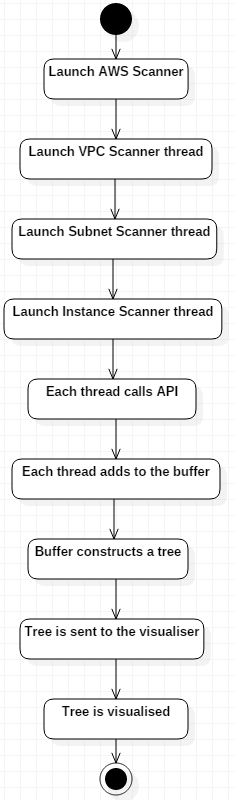
\includegraphics[width=1\textwidth] {./Diagrams/ScanNetworkSequence.png}\\[0.4cm]    
		\end{center}
	\item Get Node Information
		\begin{center}
	 	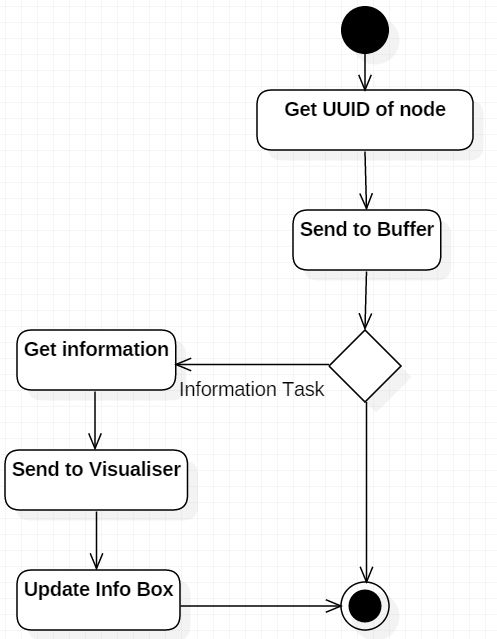
\includegraphics[width=1\textwidth] {./Diagrams/GetNodeInformationSequence.png}\\[0.4cm]
		\end{center}
	\item Scan From
		\begin{center}
			 	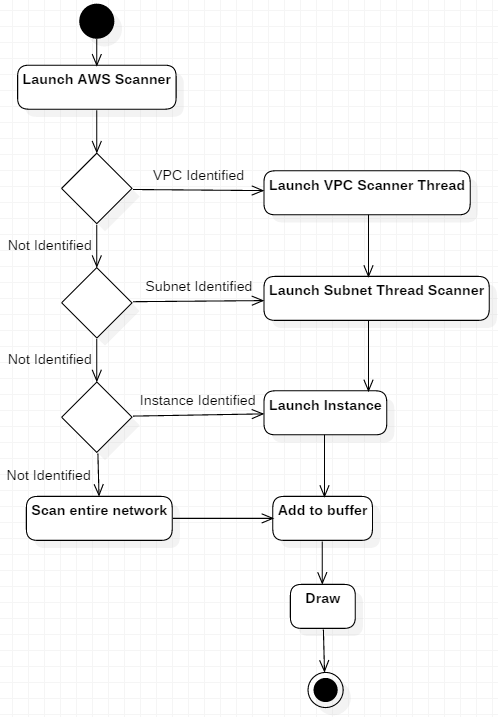
\includegraphics[width=1\textwidth] {./Diagrams/ScanFromSequence.png}\\[0.4cm]
		\end{center}
	\item Scan Region
		\begin{center}
			 	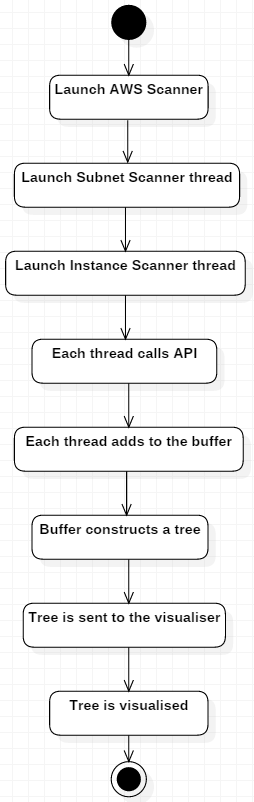
\includegraphics[width=1\textwidth] {./Diagrams/ScanRegionSequence.png}\\[0.4cm]
		\end{center}
	\item Change Scanner State
		\begin{center}
	 	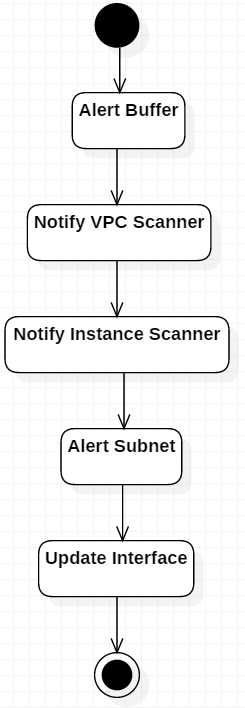
\includegraphics[width=1\textwidth] {./Diagrams/ChangeScannerStateSequence.png}\\[0.4cm]
		\end{center}
	\item Scan Instances
	\begin{center}
		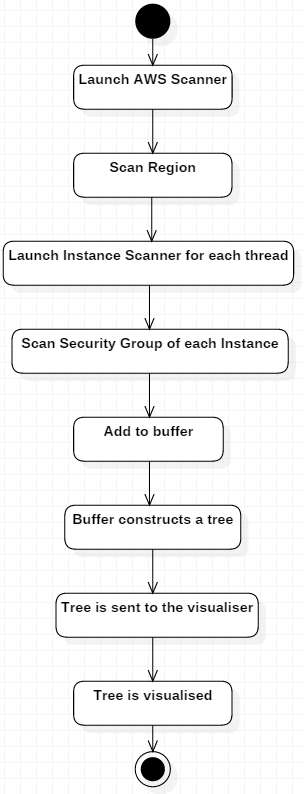
\includegraphics[width=1\textwidth] {./Diagrams/ScanInstancesSequence.png}\\[0.4cm]
	\end{center}
\end{itemize}
\subsection{Domain Model}
	\begin{center}
  	  	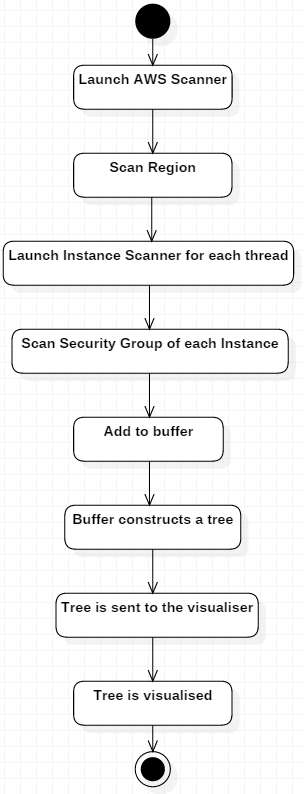
\includegraphics[width=1\textwidth] {./Diagrams/ScanInstancesSequence.png}\\[0.4cm]    
	\end{center}
\index{Vision}

\end{document}
